\section{Valutazione delle performance}
La valutazione delle performance può essere fatta su due piani differenti, a seconda dei casi:
\begin{itemize}
    \item il \textbf{tempo di risposta}, anche conosciuto come il \emph{tempo di esecuzione} o \emph{tempo di latenza}, è definito come il tempo necessario per completare un task o un job.

\item il \textbf{throughput} è l'ammontare di lavoro totale eseguito in un dato time slot, a volte chiamato \textbf{larghezza di banda}.
\end{itemize}

Lo speedup è definito come il rapporto tra il tempo di esecuzione di due programmi:
\begin{equation*}
	n=\frac{execTime_y}{execTime_x}
\end{equation*}
di solito $execTime_y$ viene sostituito dal tempo di esecuzione della versione sequenziale di un programma $P$ e $execTime_x$ con la sua versione parallelizzata.

Le misurazioni delle performance possono essere fatte a diversi livelli (considerando solo l'architettura hardware, una sua parte, o una parte di codice, o un intero programma, oppure tutto l'insieme) sfruttando funzionalità contenute in una \textbf{benchmark suite} (un insieme di tool di benchmark, come i \textbf{kernels} che sono piccoli pezzi di codice chiave presi da applicazioni reali, oppure i \textbf{toy programs} che contengono programmi, solitamente lunghi 100 linee di codice, che implementano algoritmi come la moltiplicazione tra matrici, il quicksort, e così via. Vi sono poi i \textbf{benchmark sintetici}, ovvero programmi ideati per simulare il comportamento delle applicazioni reali (come il Linpak, e il Dhrystone). La \textbf{SPEC} (Standard Performance Evaluation Corporation) è un consorzio senza scopo di lucro che stabilisce, mantiene e approva benchmark e strumenti standardizzati per valutare le prestazioni per la nuova generazione di sistemi informatici. SPEC sviluppa suite di benchmark e inoltre esamina e pubblica i risultati presentati dalle nostre organizzazioni membri e da altri licenziatari di benchmark.

Per comparare le performance di un componente hardware può essere consultata una \textbf{tabelle delle performance} dei modelli disponibili in commercio. Le informazioni più importanti riguardano i benchmark per completare un particolare task e il costo del componente hardware.

\subsection{Principio quantitativo} Per aumentare lo speedup è necessario concentrare le energie sul codice che viene eseguito più frequentemente, piuttosto che quello eseguito più raramente.

Un importante riferimento a tal proposito, è la \textbf{legge di Amdahl}
\paragraph{Legge di Amdahl.}
\begin{mdframed}
    \textit{"Il miglioramento delle prestazioni di un sistema che si può ottenere ottimizzando una certa parte del sistema è limitato dalla frazione di tempo in cui tale parte è effettivamente utilizzata"}
\end{mdframed}
Di seguito con $f_i \le 1$ (\textit{"fraction improved"}) viene indicata la frazione del tempo di esecuzione della macchina originale (o del codice originale) che può essere modificato per sfruttare i miglioramenti, mentre con $s_i \ge 1$ (\textit{"speedup improved"}) viene indicato il miglioramento ottenuto da un una modalità di esecuzione più veloce.
\begin{align}
    e_n &= e_o \cdot \left((1-f_i) + \frac{f_i}{s_i} \right) \label{eqn:execution-time-new} \\
    s_g &= \frac{e_o}{e_n}= \frac{1}{(1-f_i)+ \frac{f_i}{s_i}}\label{eqn:speedup-global}
\end{align}
Se un miglioramento può essere usato solo per una frazione dell'intero task:
\begin{equation}
    s_g = \frac{1}{(1-f_i)+\frac{f_i}{s_i}} \fcolorbox{red}{white}{$\le \frac{1}{(1-f_i)}$} \label{eqn:speedup-global-with-limit}
\end{equation}
\begin{eqnarray}
    \begin{tblr}{|c|c|}
    \hline
       e_n & \text{execution time new}
       \\
       \hline
       e_o & \text{execution time old}
       \\
       \hline
       f_i & \text{fraction improved}
       \\
       \hline
       s_i & \text{speedup improved}
       \\
       \hline
       s_g & \text{speedup global}
       \\
       \hline
    \end{tblr}
\end{eqnarray}

Lo \textbf{speedup globale} $s_g$ è uguale a $ \frac{1}{(1-f_i)+\frac{f_i}{s_i}}$ dove $1-f_i$ è la frazione non parallelizzabile, $f_i$ è la frazione parallelizzabile e $s_i$ è lo speedup che si ottiene dalla porzione parallelizzabile di codice. Lo speedup globale massimo, nel riquadro rosso (equazione \ref{eqn:speedup-global-with-limit}) si ottiene facendo tendere la $s_i$ all'infinito: \[\lim_{s_i \to \infty}{\frac{f_i}{s_i}} = 0\]
\begin{exercise}
	Si consideri un miglioramento di 10 volte più veloce della macchina originale (o del codice) ma che può essere applicato solo per il 40\% del tempo. Qual'è il guadagno totale?
\end{exercise}
\begin{solution}
	Traendo i dati dal problema, si ottiene che lo $s_i = 10$ e che $f_i = 40\% = 0,4$. Sostituendo alla formula \ref{eqn:speedup-global} si ottiene
	\begin{equation*}
		s_g = \frac{1}{(1-0.4)+\frac{0.4}{10}} = \frac{1}{0.6+0.04} = \frac{1}{0.64} = \frac{100}{64} = 1.56
	\end{equation*}

	Lo speedup ottenuto è di 1.56.
\end{solution}

\begin{exercise}
	Si consideri una CPU che è stata aggiornata per avere i seguenti cambiamenti:
	\begin{enumerate}
		\item aumentare la velocità di un fattore pari a 5 senza interessare le performance del sistema I/O;
		\item il costo è 5 volte superiore al precedente;
		\item la CPU può essere utilizzata per il 50\% del tempo totale, mentre il rimanente viene impiegato per operazioni di I/O;
		\item il costo della CPU è $\frac{1}{3}$ del costo della macchina.
	\end{enumerate}
	Questo investimento, è conveniente?
\end{exercise}
\begin{solution}
	Lo $s_i = 5$, la $f_i = 50\% = 0.5$. Lo speedup globale è:
	\begin{equation*}
		s_g = \frac{1}{(1-0.5)+\frac{0.5}{5}}=\frac{1}{0.5+0.1} = \frac{10}{6} = 1.67
	\end{equation*}
	il costo è aumentato di:
	\begin{equation*}
		c = 1 \cdot \frac{2}{3} + 5 \cdot \frac{1}{3} =\frac{7}{3} = 2.33
	\end{equation*}
	Dato che il costo è superiore al rendimento ottenuto $ c = 2.33 >  s_g = 1.67 $ non è conveniente fare l'aggiornamento del processore.
\end{solution}

\begin{exercise}
	Si vuole riscrivere un programma su un'architettura MIMD con 100 processori. L'obbiettivo è di ridurre il tempo di esecuzione di 80 volte rispetto a quello precedente su un'architettura SIMD. Qual'è la frazione del programma originale che può restare sequenziale?
\end{exercise}
\begin{solution}
	Dati disponibili: $s_i = 80$. Si sa che $f_i$ è un'incognita.
\end{solution}












%%%%%%%%%%%%%%%%%%%%%%%%%%%%%%%%%%%%%%%%%%%%%%%%%%%%%%%%%%%%%%%%%%%%%%%%

\subsection{Tempo di esecuzione} Il tempo di esecuzione viene usato per misurare le performance di un computer: l'architettura che performa lo stesso ammontare di tempo in meno tempo è la più veloce. Il \textbf{tempo di risposta rappresenta} la latenza per completare una task includendo accessi al disco, accessi alla memoria e le operazioni di input/output. Il \textbf{CPU time} corrisponde invece solamente al tempo utente pù il tempo di sistema della CPU (non include il tempo di attesa delle operazioni di I/O o di esecuzioen delle altre task, ad esempio).
Il CPU time è calcolato come segue:
\begin{align*}
\text{CPU\_time} &= \text{Cicli di clock della CPU per una task} * \text{tempo di un ciclo di clock}\\
&= \frac{\text{Cicli di clock della CPU per una task}}{\text{Frequenza di clock}}
\end{align*}

I Cicli di clock per istruzione (CPI) medi vengono calcolati come segue:
\begin{align*}
\text{CPI} &= \frac{\text{Cicli di clock della CPU per una task}}{\text{Numero di istruzioni}}\\
\text{CPU time} &= \text{N di istruzioni} * \text{CPI} * \text{durata di un ciclo di clock}\\
&= \frac{\text{N di istruzioni} * \text{CPI}}{\text{Frequenza di clock}}\\
T_{CPU} &= CI * CPI * T_{CLOCK} = \frac{CI * CPI}{f_{CLOCK}}
\end{align*}

La relazione tra le varie metriche è visibile di seguito:
\begin{align*}
    \frac{\text{istruzioni}}{\text{task}} * \frac{\text{cicli di clock}}{\text{istruzione}} * \frac{\text{secondi}}{\text{cicli di clock}}= \frac{\text{secondi}}{\text{task}} = \text{CPU time}
\end{align*}

Il tempo di CPU dipende da 3 parametri:
\begin{itemize}
    \item \textbf{Ciclo di clock (o frequenza)}: dipende dalla tecnologia, quindi l'unico modo per migliorare questo parametro consiste nel sostituire l'architettura;
    \item \textbf{CPI}: se vogliamo migliorare il numero medio di istruzioni per clock, l'unico come è migliorare l'organizzazione e l'instruction set del sistema che si usa -> possiamo avere architetture che forniscono poche istruzioni, che però sono molto complesse alla base e quindi richiedono più tempo per essere terminate;
    \item \textbf{Numero di istruzioni}: il numero di istruzioni usate da un programma dipende dall'instruction set architecture e dalla tecnologia del compilatore. Un buon compilatore permette idealmente di avere un codice finale con meno istruzioni (ovviamente un fattore importante rimane la capacità del programmatore).
\end{itemize}

Il numero totale di cicli di clock per una task si calcola come segue:
\begin{align*}
    \text{Cicli di clock della CPU} = \sum^n_{i=1} (CPI_i * I_i)
\end{align*}
dove:
\begin{itemize}
    \item $I_i$ rappresenta il numero di volte in cui l'istruzione $I$ è stata eseguita in una task;
    \item $CPI_i$ rappresenta il numero medio di cicli di clock spesi per una generica istruzione.
\end{itemize}

Date queste misure, il CPU time può essere riscritto come:
\begin{align*}
    T_{CPU} = \sum^n_{i = 1} (CPI_i * I_i) * T_{CLOCK}
\end{align*}


\subsection{MIPS e GIPS}
Con le sigle MIPS e GISP si intendono rispettivamente milioni di microistruzioni per secondo e miliardi di microistruzioni per secondo, dove:
\begin{align*}
    MIPS &= \frac{\text{N di istruzioni}}{\text{Tempo di esecuzione} * 10^6}\\
    &= \frac{\text{frequenza di clock}}{CPI * 10^6}
\end{align*}

Il tempo di esecuzione diventa:
\begin{align*}
    \text{Tempo di esecuzione} = \frac{\text{N di istruzioni}}{MIPS * 10^6}
\end{align*}

Poiché MIPS rappresenta la frequenza di operazioni per unità di tempo, le performance per la macchina più veloce cha ha alti valori MIPS può essere specificata come l'inversa del tempo di esecuzione. Il vantaggio del MIPS è che è semplice da capire: le macchine più veloci hanno valori MIPS più alti. 

La metrica MIPS presenta comunque una serie di problematiche:
\begin{itemize}
    \item Il valore dipende dall'instruction set, quindi è difficile da comparare con macchine che hanno diversi instruction set;
    \item Varia in base al programma considerato;
    \item Varia in modo inversamente proporzionale alla performance.
\end{itemize}

La limitazione principale di questa misura è che non considera il tipo di istruzioni eseguite. Ad esempio, le operazioni su interi sono generalmente più







Se ci interessa misurare nello specifico le performance relative alle operazioni floating-point possiamo utilizzare la metrica GFLOPS, che sta per \textbf{billion of FP instructions per second} (dove FP indica le operazioni floating-point):
\begin{align*}
    GFLOPS = \frac{\text{N di \textbf{operazioni} FP in un programma}}{\text{Tempo di esecuzione} * 10^9}
\end{align*}

Ovviamente questa metrica non può essere usata in contesti diversi da quelli legati alle operazioni FP. Essendo basata su operazioni piuttosto che istruzioni, i FLOPS sono concepiti per essere un buon metodo di confronto tra le varie architetture. L'ipotesi è che stesso programma, lanciato su differenti architetture, esegue un diverso numero di istruzioni, ma lo stesso numero di operazioni floating-point. Le operazioni FP non sono considerate tra diverse architetture; il GFLOPS cambia cambiando il rapporto tra le operazioni intere e FP oppure cambiando il mix di operazioni FP veloci e lente.

Il \textbf{Normalized GFLOPS} prevede di associare un bias, con funzione di peso, ad ogni operazione FP, come mostrato in figura \ref{fig:normalized-gflops}.
\begin{figure}[th]
	\centering
	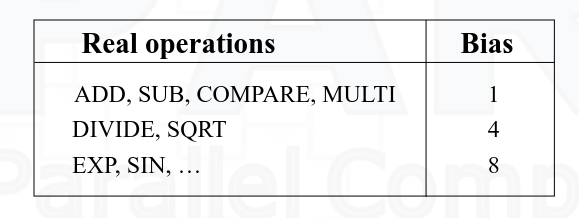
\includegraphics[width=0.7\linewidth]{img/normalized-gflops.png}
	\caption{Esempio di bias per operazioni FP.}
	\label{fig:normalized-gflops}
\end{figure}

Un frammento di codice con operazioni un'operazione ADD, una DIVIDE e una SIN, si calcola avere 12 operazioni FP normalizzate.
















